\documentclass[letterpaper]{article}
\usepackage[margin=1in]{geometry}
\usepackage[utf8]{inputenc}
\usepackage{textcomp}
\usepackage{amssymb}
\usepackage{natbib}
\usepackage{graphicx}
\usepackage{gensymb}
\usepackage{amsthm, amsmath, mathtools}
\usepackage[dvipsnames]{xcolor}
\usepackage{enumerate}
\usepackage{mdframed}
\usepackage[most]{tcolorbox}
\usepackage{csquotes}
% https://tex.stackexchange.com/questions/13506/how-to-continue-the-framed-text-box-on-multiple-pages

\tcbuselibrary{theorems}

\newcommand{\R}{\mathbb{R}}
\newcommand{\Z}{\mathbb{Z}}
\newcommand{\N}{\mathbb{N}}
\newcommand{\Q}{\mathbb{Q}}
\newcommand{\C}{\mathbb{C}}
\newcommand{\code}[1]{\texttt{#1}}
\newcommand{\mdiamond}{$\diamondsuit$}
\newcommand{\PowerSet}{\mathcal{P}}
\newcommand{\Mod}[1]{\ (\mathrm{mod}\ #1)}
\DeclareMathOperator{\lcm}{lcm}

%\newtheorem*{theorem}{Theorem}
%\newtheorem*{definition}{Definition}
%\newtheorem*{corollary}{Corollary}
%\newtheorem*{lemma}{Lemma}
\newtheorem*{proposition}{Proposition}


\newtcbtheorem[number within=section]{theorem}{Theorem}
{colback=green!5,colframe=green!35!black,fonttitle=\bfseries}{th}

\newtcbtheorem[number within=section]{definition}{Definition}
{colback=blue!5,colframe=blue!35!black,fonttitle=\bfseries}{def}

\newtcbtheorem[number within=section]{corollary}{Corollary}
{colback=yellow!5,colframe=yellow!35!black,fonttitle=\bfseries}{cor}

\newtcbtheorem[number within=section]{lemma}{Lemma}
{colback=red!5,colframe=red!35!black,fonttitle=\bfseries}{lem}

\newtcbtheorem[number within=section]{example}{Example}
{colback=white!5,colframe=white!35!black,fonttitle=\bfseries}{def}

\newtcbtheorem[number within=section]{note}{Important Note}{
        enhanced,
        sharp corners,
        attach boxed title to top left={
            xshift=-1mm,
            yshift=-5mm,
            yshifttext=-1mm
        },
        top=1.5em,
        colback=white,
        colframe=black,
        fonttitle=\bfseries,
        boxed title style={
            sharp corners,
            size=small,
            colback=red!75!black,
            colframe=red!75!black,
        } 
    }{impnote}
\usepackage[utf8]{inputenc}
\usepackage[english]{babel}
\usepackage{fancyhdr}
\usepackage[hidelinks]{hyperref}

\pagestyle{fancy}
\fancyhf{}
\rhead{Math 103B}
\chead{Monday, February 28, 2022}
\lhead{Lecture 21}
\rfoot{\thepage}

\setlength{\parindent}{0pt}

\begin{document}

\section{Vector Space}
We continue our discussion about \textbf{vector spaces}.

\subsection{Basis}
\begin{definition}{Basis}{}
    Let $V$ be a vector space over a field $F$. A subset $B$ of $V$ is called a \textbf{basis} for $V$ if $B$ is linearly independent and every element of $V$ is a linear combination of elements of $B$ (i.e. $B$ spans $V$).
\end{definition}
\textbf{Fact:} Every $v \in V$ is a unique linear combination of basis vectors. 

\subsubsection{Example 1: Standard Basis Vector}
Consider the standard basis vector of $\R^n$: 
\[\left\{
    \begin{bmatrix}
        1 \\ 0 \\ 0 \\ \vdots \\ 0 
    \end{bmatrix}, \begin{bmatrix}
        0 \\ 1 \\ 0 \\ \vdots \\ 0 
    \end{bmatrix}, \begin{bmatrix}
        0 \\ 0 \\ 1 \\ \vdots \\ 0 
    \end{bmatrix}, \begin{bmatrix}
        0 \\ 0 \\ 0 \\ \vdots \\ 0 
    \end{bmatrix}, \begin{bmatrix}
        0 \\ 0 \\ 0 \\ \vdots \\ 1 
    \end{bmatrix}
\right\}\]
A classic example is $\R^2$, which has basis $\left\{\begin{bmatrix}
    0 \\ 1
\end{bmatrix}, \begin{bmatrix}
    1 \\ 0
\end{bmatrix}\right\}$. Here, we can visualize this by looking at a graph.
\begin{center}
    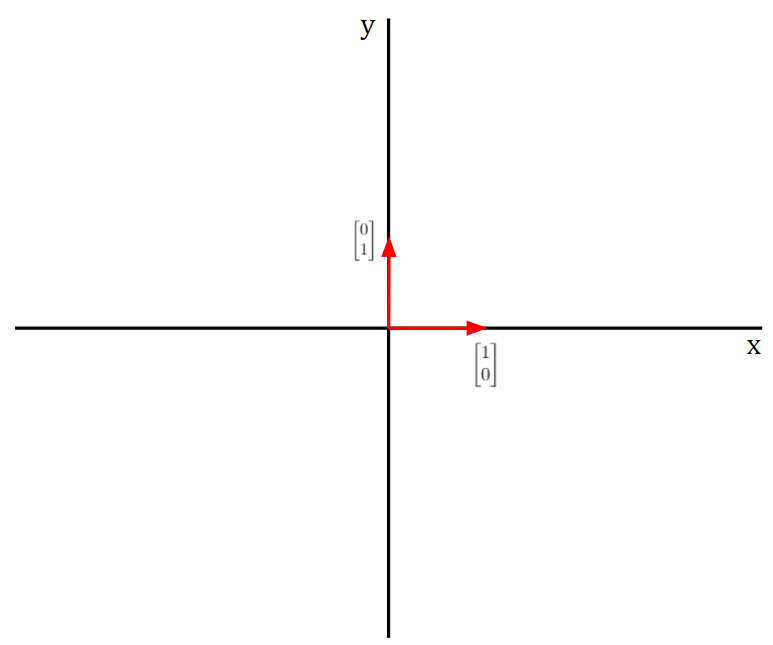
\includegraphics[scale=0.7]{../assets/r2.png}
\end{center}
Here, the idea is that we can reach any point in this graph uniquely by multiplying $\begin{bmatrix}
    0 \\ 1
\end{bmatrix}$ and $\begin{bmatrix}
    1 \\ 0
\end{bmatrix}$ by the appropriate scalar constants. 

\subsubsection{Example 2: Vector Space over Rational Numbers}
We claim that $\Q[x] / I$, where $I = \cyclic{x^3 + x + 1}$, is a vector space over $\Q$. To see this, we note the following: 
\begin{itemize}
    \item This is a ring, and in fact is a field since $x^3 + x + 1$ is irreducible. Therefore, addition is implied, and since this is a field, it is abelian. 
    \item Consider the set of all cosets 
    \[\left\{ax^2 + bx + c + I \mid a, b, c \in \Q\right\}\]
    If $r \in \Q$, then $r(ax^2 + bx + c + I) = rax^2 + rbx + rc + \cyclic{x^2 + x + 1}$. So, scalar multiplication is satisfied. 
    \item The set $\{1 + I, x + I, x^2 + I\}$ is a basis for this vector space. Once again, to see this, we show that the properties of a basis are satisfied. 
    \begin{itemize}
        \item The linear combinations of these vectors clearly span the entire set. That is, 
        \[a_0 (1 + I) + a_1 (x + I) + a_2 (x^2 + I) = a_0 + a_1 x + a_2 x^2 + I\]

        \item To see linear independence, we note that 
        \[a_0 (1 + I) + a_1 (x + I) + a_2 (x^2 + I) = 0 + I\]
        But we see that
        \[a_0 + a_1 x + a_2 x^2 + I = 0 + I\]
        However, this implies that 
        \[a_0 + a_1 x + a_2 x^2 \in I\]
        This further implies that 
        \[a_0 + a_1 x + a_2 x^2 = (x^3 + x + 1) g(x)\]
        But note that if $g(x)$ is not zero, then $(x^3 + x + 1) g(x)$ will have degree 3 or larger, but the left-hand side will never have this. This means that  
        \[g(x) = 0\]
        This implies that $a_0 = a_1 = a_2 = 0$.
    \end{itemize}
\end{itemize}

\subsection{Invariance of Basis Size}
\begin{theorem}{}{}
    If $\{u_1, u_2, \dots, u_m\}$ and $\{w_1, w_2, \dots, w_n\}$ are bases of $V$, then $m = n$.
\end{theorem}
\textbf{Facts:} Let $V$ be a finite dimensional vector space.
\begin{itemize}
    \item Every spanning set contains a basis. 
    \item If $\dim V = n$, a spanning set has size $\geq n$ with equality if and only if it is a basis. 
    \item Every linearly independent set is contained in a basis. 
    \item If $\dim V = n$, a linearly independent set has size $\leq n$ with equality if and only if it is a basis. 
\end{itemize}

\begin{mdframed}[]
    \begin{proof}
        Suppose towards a contradiction that $m \neq n$, WLOG $m < n$. The $u$'s span $V$. So, we write $w_1 = a_1 u_1 + \dots + a_m u_m$. Here, we're starting the process of expressing one basis in terms of another basis. We claim that $w_1 \neq 0$. Then, $a_i \neq 0$ for some $i$. WLOG let $a_1 \neq 0$. Then, we can solve for $u_1$. In particular, since the scalars are from a field, we can use inverses like so 
        \[u_1 = a_{1}^{-1} w_1 - a_{1}^{-1} a_2 u_2 - \dots - a_{1}^{-1} a_m u_m.\]
        This implies that 
        \[u_1 \in \text{Span}\{w_1, u_2, \dots, u_m\}.\]
        We now do the same thing for $w_2$. So 
        \[w_2 = b_1 w_1 + b_2 u_2 + \dots + b_m u_m\]
        Evidently, we end up with 
        \[u_2 \in \text{Span}\{w_1, w_2, u_3, \dots, u_m\}.\]
        and $u_1 \in \text{Span}\{w_1, w_2, u_3, \dots, u_m\}$. By repeating this process, repeating $m$ times, we get 
        \[u_1, \dots, u_m \in \text{Span}\{w_1, \dots, w_m\}.\]
        We note that there is at least one more $w$ to account for. So 
        \[w_{m + 1} = c_1 u_1 + \dots + c_m u_m \in \text{Span}\{w_1, w_2, \dots, w_m\}.\]
        This is a contradiction as we have a dependent relationship. 
    \end{proof}
\end{mdframed}


\subsection{Dimension of a Vector Space}
\begin{definition}{Dimension}{}
    A vector space $V$ has dimension $n$, written $\dim V = n$, if $V$ has a basis with $n$ vectors.
\end{definition}
\textbf{Remarks:} 
\begin{itemize}
    \item Sometimes, we write $\dim_{F} V = n$, where $F$ is the field used.
    \item For completion, $\dim \{0\} = 0$.
    \item $\dim_{F} F[x] / \cyclic{f(x)} = \deg f(x)$.  
    \item $\left| \F_p [x] / \cyclic{f(x)} \right| = p^n$ where $\deg f(x) = n$. 
    \item If $V$ is an $n$-dimensional vector space over $\F_p$, then $|V| = p^n$. 
\end{itemize}

\subsubsection{Example 1: Dimension}
What is $\dim \Q[x] / \cyclic{x^3 + x + 1}$? 

\begin{mdframed}[]
    This has dimension 3 because the basis, $\{1 + I, x + I, x^2 + I\}$, has length 3.
\end{mdframed}

\subsubsection{Example 2: Dimension}
What is $\dim \R[x] / \cyclic{x^2 + 1}$? 

\begin{mdframed}[]
    This has dimension 2.
\end{mdframed}


\end{document}